\documentclass[a4paper]{article}

%% Language and font encodings
\usepackage[english]{babel}
\usepackage[utf8]{inputenc}
\usepackage[T1]{fontenc}
\usepackage{authblk}
\usepackage[export]{adjustbox}
\usepackage{booktabs}
\usepackage{ae,aecompl}
%% Sets page size and margins
\usepackage[a4paper,top=3cm,bottom=2cm,left=3cm,right=3cm,marginparwidth=1.75cm]{geometry}

%% Useful packages
\usepackage{pgfplots}
\pgfplotsset{compat=1.12}
\usepackage[group-separator={,}]{siunitx}
\usepackage{amsmath}
\usepackage{wrapfig}
\usepackage{amsthm}
\usetikzlibrary{arrows,automata}
\usepackage{algpseudocode}
\usepackage{graphicx}
\usepackage{algorithm}
\usepackage{breqn}
\usepackage{algpseudocode}
\usepackage{float}
\usepackage{tikz}
\usepackage{pifont}% http://ctan.org/pkg/pifont
\newcommand{\cmark}{\ding{51}}%
\newcommand{\xmark}{\ding{55}}%
\usepackage{eufrak}
\usepackage{caption}
\usepackage{subcaption}
\usepackage{listings}
\usepackage[toc,page]{appendix}
\usepackage{color}
\definecolor{lightgray}{rgb}{.9,.9,.9}
\definecolor{darkgray}{rgb}{.4,.4,.4}
\definecolor{purple}{rgb}{0.65, 0.12, 0.82}
\floatname{algorithm}{Procedure}
\renewcommand{\algorithmicrequire}{\textbf{Input:}}
\renewcommand{\algorithmicensure}{\textbf{Output:}}

\lstdefinelanguage{JavaScript}{
	keywords={typeof, contract, struct, new, true, false, catch, function, return, null, catch, switch, var, if, in, while, do, else, case, break},
	keywordstyle=\color{blue}\bfseries,
	ndkeywords={class, export, boolean, throw, implements, import, this},
	ndkeywordstyle=\color{darkgray}\bfseries,
	identifierstyle=\color{black},
	sensitive=false,
	comment=[l]{//},
	morecomment=[s]{/*}{*/},
	commentstyle=\color{purple}\ttfamily,
	stringstyle=\color{red}\ttfamily,
	morestring=[b]',
	morestring=[b]"
}

\lstset{
	language=JavaScript,
	backgroundcolor=\color{lightgray},
	extendedchars=true,
	basicstyle=\footnotesize\ttfamily,
	showstringspaces=false,
	showspaces=false,
	numbers=left,
	numberstyle=\footnotesize,
	numbersep=9pt,
	tabsize=2,
	breaklines=true,
	showtabs=false,
	captionpos=b
}

\usepackage{graphicx}
\usepackage[
n,
operators,
advantage,
sets,
adversary,
landau,
probability,
notions,	
logic,
ff,
mm,
primitives,
events,
complexity,
asymptotics,
keys]{cryptocode}
\usepackage[colorinlistoftodos]{todonotes}
\usepackage[colorlinks=true, allcolors=blue]{hyperref}

\theoremstyle{definition}
\newtheorem{definition}{Definition}[section]

\newcommand{\Mod}[1]{\ (\mathrm{mod}\ #1)}

\def\bitcoinA{%
	\leavevmode
	\vtop{\offinterlineskip %\bfseries
		\setbox0=\hbox{B}%
		\setbox2=\hbox to\wd0{\hfil\hskip-.03em
			\vrule height .3ex width .15ex\hskip .08em
			\vrule height .3ex width .15ex\hfil}
		\vbox{\copy2\box0}\box2}}

\DeclareMathOperator{\EX}{\mathbb{E}}% expected value
\providecommand{\keywords}[1]{\textbf{\textit{Keywords:}} #1}

\renewcommand{\lstlistingname}{Figure}% Listing -> Algorithm
\renewcommand{\lstlistlistingname}{List of \lstlistingname s}% List of Listings -> List of Algorithms

\newcommand{\smallsim}{\smallsym{\mathrel}{\sim}}

\makeatletter
\newcommand{\smallsym}[2]{#1{\mathpalette\make@small@sym{#2}}}
\newcommand{\make@small@sym}[2]{%
	\vcenter{\hbox{$\m@th\downgrade@style#1#2$}}%
}
\newcommand{\downgrade@style}[1]{%
	\ifx#1\displaystyle\scriptstyle\else
	\ifx#1\textstyle\scriptstyle\else
	\scriptscriptstyle
	\fi\fi
}
\makeatother


\title{Topological Analysis of Bitcoin's Lightning Network }
\author[1]{István András Seres}
\author[1]{Dániel A. Nagy}
\author[1]{Péter Burcsi}
\affil[1]{Department of Computer Algebra, Eötvös Loránd University}
\begin{document}
\maketitle

\begin{abstract}
Bitcoin's Lightning Network (LN) is a scalability solution for Bitcoin, which allows transactions to be issued with negligible fees and settle transactions instantly at scale. In order to use LN funds need to be locked in payment channels on the Bitcoin blockchain (Layer-1), that one may use them in LN (Layer-2). LN is comprised of many payment channels forming a payment channel network. A few payment channels already enable anyone to efficiently, securely and privately route payments across the whole network. In this paper we argue that LN's current topological properties largely harms its value proposition and potential.  
\end{abstract}
\keywords{Bitcoin, Lightning Network, Network Topology, Payment Channel Network}

\section{Introduction}
Recently the Bitcoin \cite{nakamoto2008bitcoin} network celebrated its 10th anniversary. During these years Bitcoin gained a huge popularity due to its publicly verifiable, decentralized, permissionless and censorship-resistant nature. This tremendous popularity and increasing interest in Bitcoin pushed its network's throughput to its limits. Without further advancements, the Bitcoin network can only settle $7$ transactions per second (tps), while mainstream centralized payment providers such as Visa and Mastercard can process approximately \num[group-separator={,}]{40000} tps in peak hours. Moreover one might need to pay large transaction fees on the Bitcoin network, while also need to wait 6 new blocks to be published in order to be certain enought that the transaction is included in the blockchain.

\begin{wrapfigure}{r}{0.7\textwidth}
	\begin{center}
		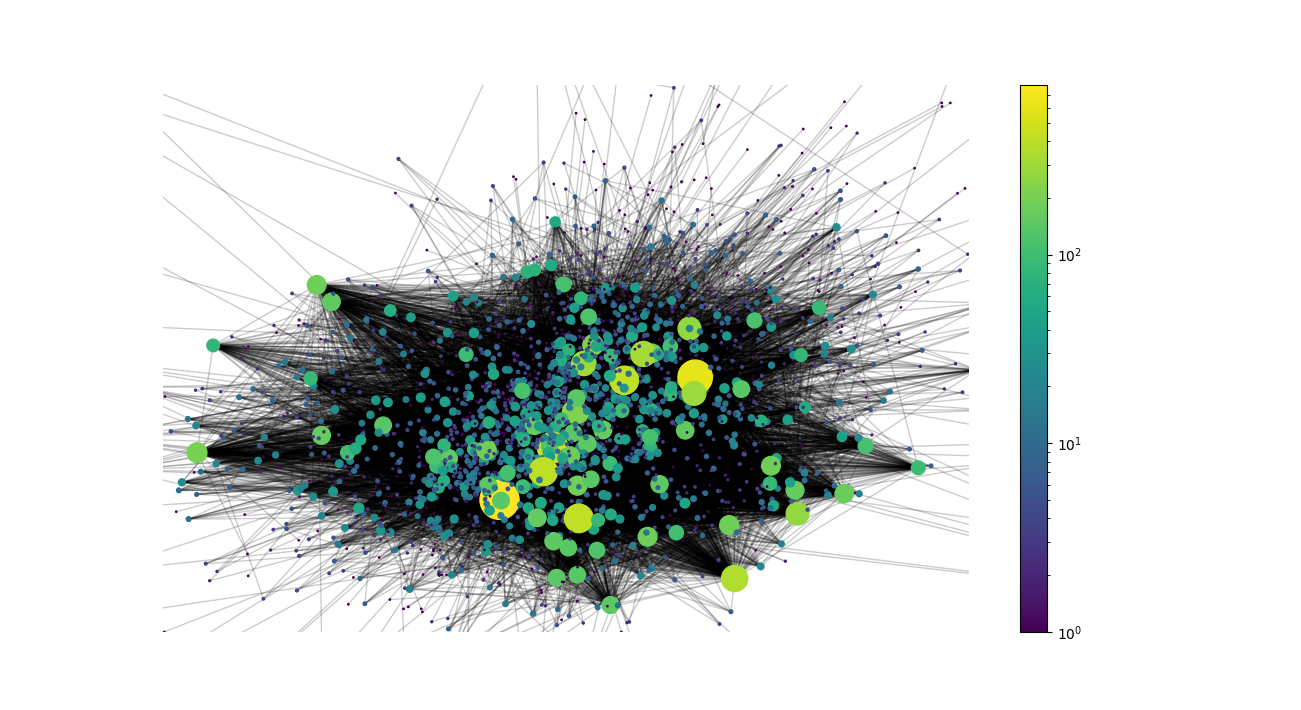
\includegraphics[width=0.9\textwidth]{LNtopology.png}
	\end{center}
	\caption{LN's topology. Nodes with higher degree are highlighted with lighter colors}
	\vspace{-10pt}
\end{wrapfigure}

To alleviate these scalability issues the Lightning Network (LN) is designed in 2016 \cite{poon2016bitcoin}, and launched in 2018, January. The main insight of LN is that transactions can be issued also off-blockchain in a trust-minimized manner achieving instant transaction confirmation times with negligible fees, whilst retaining the security of the underlying blockchain. 

Bidirectional payment channels can be formed on-chain using a construction called Hashed Timelock Contracts (HTLC). Later several payments can take place in a payment channel. The main advantage of payment channels is that one can send and receive thousands of payments with essentially only 2 on-chain transations: the opening and closing channel transactions.

Using these payment channels as building blocks one might establish a payment channel network, where it is not necessary to have direct payment channels between nodes to transact with each other, but they could simply route their payments through other nodes' payment channels.
Such a network can be built, because LN achieves payments to be made without any counterparty risk, however efficient and privacy-preserving payment routing remains a challenging algorithmic task \cite{roos2017settling}.    

\textbf{Our contributions.} We empirically measure and describe LN's topology and show that it is utterly centralized and fragile against both random failures and targeted attacks. These findings suggest that LN, unlike Bitcoin, is far from being reliable, censorship-resistant, decentralized and private.
\section{Lightning Network's Topology}
\begin{wrapfigure}[18]{r}{5.5cm}
	\begin{tabular}{ | l | c | }
		\hline
		Number of nodes & $2344$  \\ \hline
		Number of payment channels & $16617$  \\ \hline
		Connected components & $2$  \\ \hline
		Density & $0.00605$ \\ \hline
		Total BTC held in LN & $543.61855$\bitcoinA\\ \hline
		s-metric& $0.6878$ \\ \hline
		Maximal independent set & $1564$ \\ \hline
		Bridges & $530$ \\ \hline
		Diameter & $6$ \\ \hline
		Radius & $3$ \\ \hline
		Transitivity& $0.1046$\\ \hline
		Average clustering coefficient&$0.304$ \\ \hline
		Degree assortativity& $-0.2690$ \\ \hline
	\end{tabular}
	\caption{LN at a glance: basic properties of the LN graph.}\label{fig:properties}
\end{wrapfigure}

LN can be described as a weighted graph $G=(V,E)$, where $V$ is the set of LN nodes and $E$ is the set of bidirectional payment channels between these nodes. We took a snapshot\footnote{https://graph.lndexplorer.com} of LN's topology on the 10th birthday of Bitcoin, 2019 January 3rd. In the following we are going to analyze this dataset.

LN gradually increased adoption and attraction throughout 2018, which resulted in 3 independent client implementations and \num[group-separator={,}]{2344} nodes joining LN as of 2019, January 3rd. The density of a graph is defined as $D=\frac{2\mid E\mid}{\mid V\mid \mid V-1\mid}$  which is the ratio of present and potential edges. As it is shown in Figure \ref{fig:properties}. LN is quite a parse graph. This is further justified by the fact that LN has \num[group-separator={,}]{530} bridges, edges which deletion increases the number of connected components. Although LN is consisted of $2$ components, the second component has only $3$ nodes. The low transitivity, fraction of present and possible triangles in the graph, highlights the sparseness of LN as well.

However LN also exhibits somewhat scale-free properties as the s-metric suggests. S-metric was first introduced by Lun Li et al. in \cite{li2005towards} and defined as $s(G)=\sum_{(u,v)\in E}deg(u)deg(v)$. The closer to $1$  s-metric of $G$ is, the more scale-free the network. Diameter and radius of LN suggests that LN is a small world. Somewhat scale-freeness is also exhibited in the degree distribution of LN. Majority of nodes have very few payment channels, although there are a few hubs who have significantly more connections as it can be seen in Figure~\ref{fig:degreedist}.

\begin{wrapfigure}{r}{0.6\textwidth}
	\caption{LN's degree distribution}\label{fig:degreedist}
	\begin{center}
		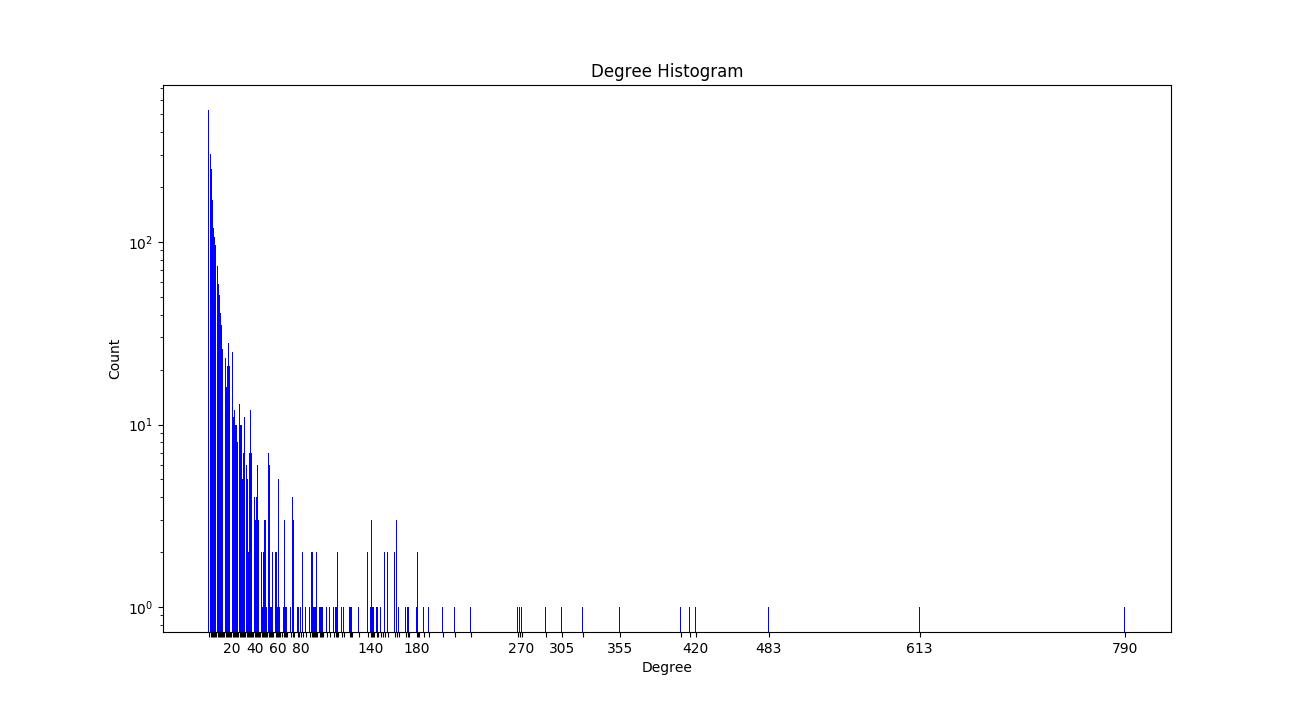
\includegraphics[width=0.85\textwidth]{degreehistogramlogscale.png}
	\end{center}	
\end{wrapfigure}

Negative degree assortativity of the graph indicates that on average low degree nodes tend to connect to high degree nodes rather than low degree nodes \cite{newman2002assortative}. Such a dissortative property hints a hub and spoke network structure, which is also reflected in the degree distribution, see Figure~\ref{fig:degreedist}.



\section{Robustness of LN}
\subsection{Random Failures}
\subsection{Targeted attacks}
\begin{figure}[h]
	\centering
	\begin{minipage}{.5\textwidth}
		\centering
		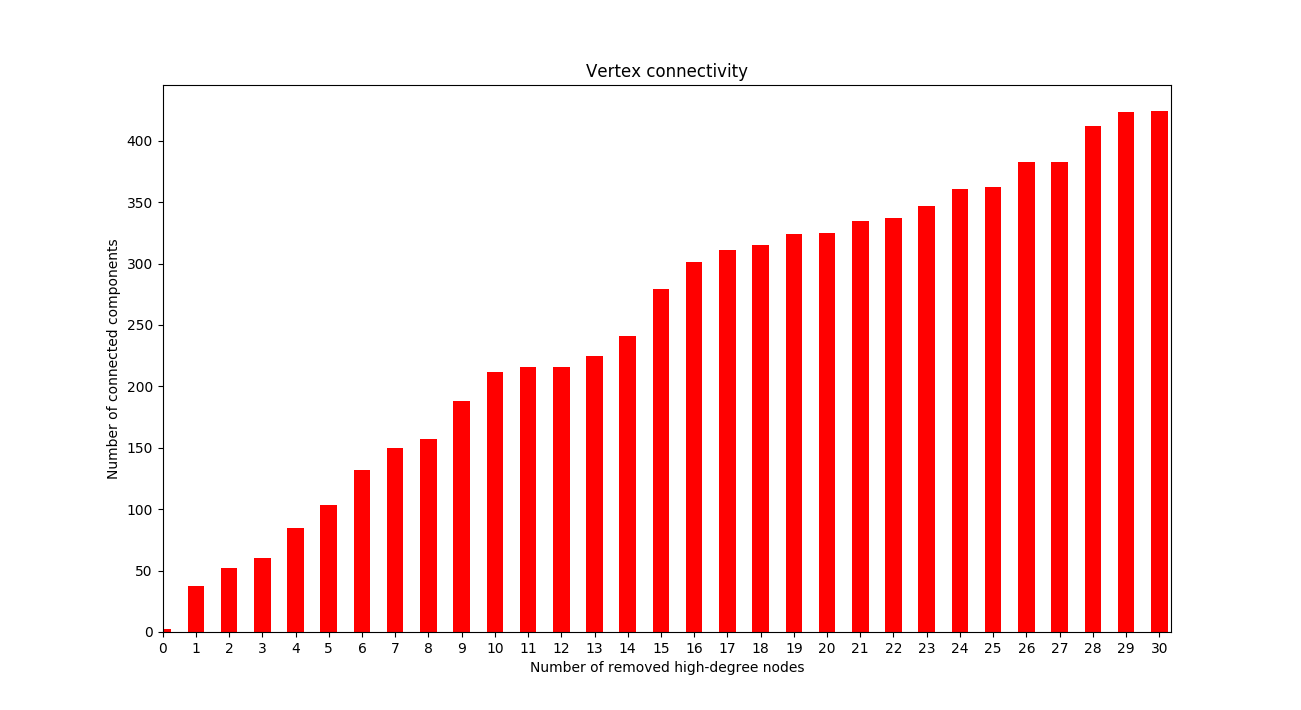
\includegraphics[width=\linewidth]{vertexConnectivity.png}
		\captionof{figure}{LN's vertex connectivity}
		\label{fig:test1}
	\end{minipage}%
	\begin{minipage}{.5\textwidth}
		\centering
		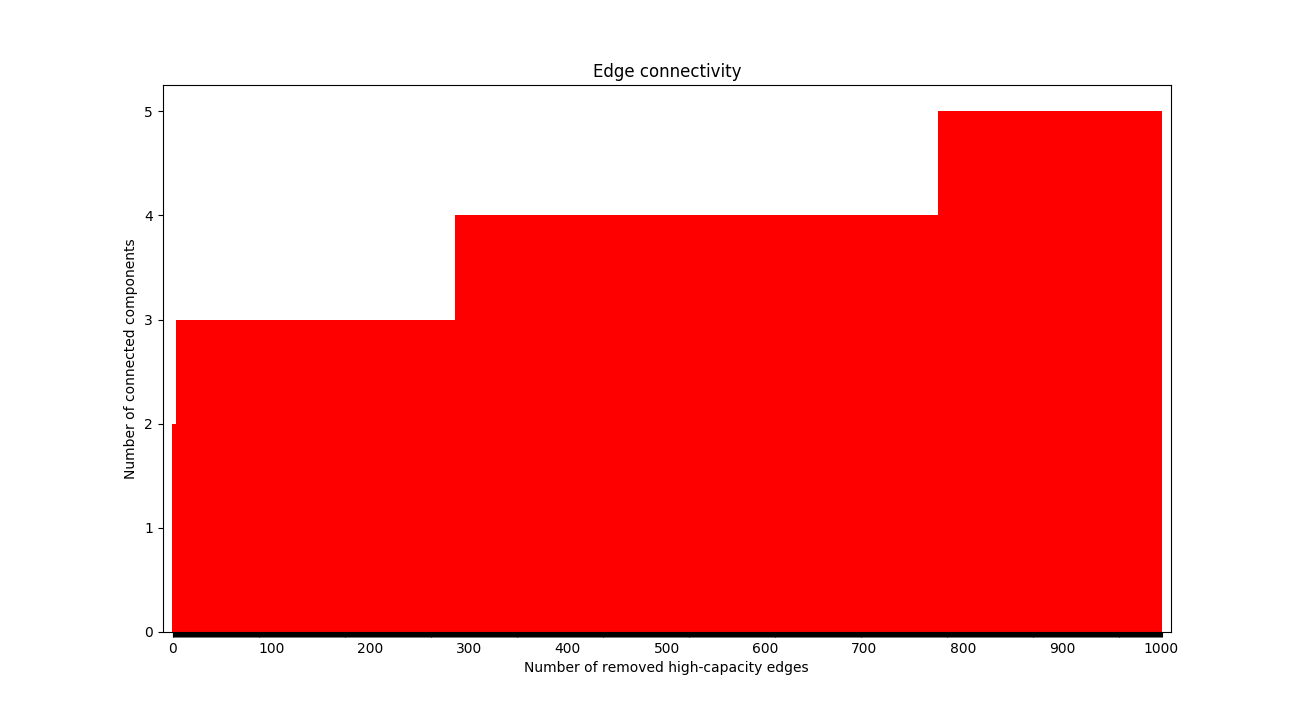
\includegraphics[width=\linewidth]{edgeConnectivity.png}
		\captionof{figure}{LN's edge connectivity}
		\label{fig:test2}
	\end{minipage}
\end{figure}

\subsection{Fixing LN's resilience against attacks}
percolation threshold
\section{Privacy}
topological anomalies have privacy implications, low usage of tor, even tor can not help
\section{Conclusion}
\section{Acknowledgements}

\bibliographystyle{plain}
\bibliography{sample}

\end{document}
